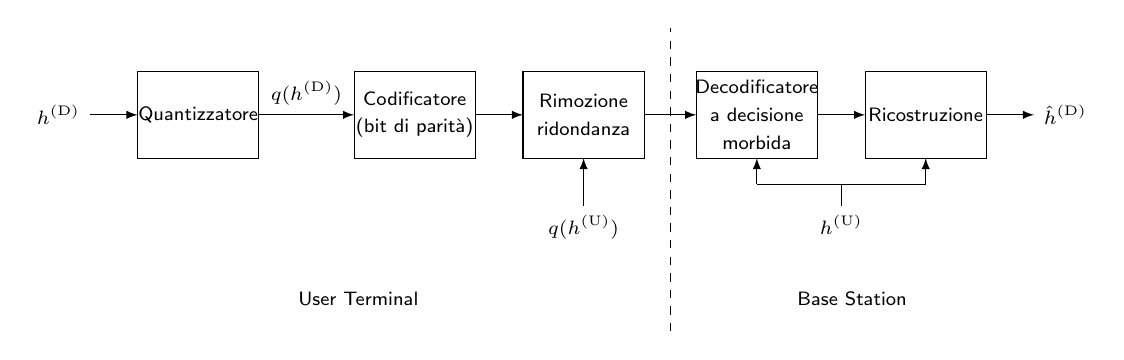
\begin{tikzpicture}[scale=0.55,>=latex]
    \tikzstyle{every node}=[font=\fontsize{6.8}{10}\sffamily]

    % Coding at UT
    \draw[->] (1.1,5) node[left]{\(\bm{h}^\mathrm{(D)}\)} -- (2.2,5);

    \draw (2.2,4) rectangle (5,6)
    node[midway,align=center]{Quantizzatore};

    \draw[->] (5,5) -- (7.2,5)
    node[above,midway]{\(q(\bm{h}^\mathrm{(D)})\)};

    \draw (7.2,4) rectangle (10,6)
    node[midway,align=center]{Codificatore \\ (bit di parità)};

    \draw[->] (10,5) -- (11.1,5);

    \draw (11.1,4) rectangle (13.9,6)
    node[midway,align=center]{Rimozione \\ ridondanza};

    \draw[->] (12.5,2.9) node[below]{\(q(\bm{h}^\mathrm{(U)})\)} -- (12.5,4);

    % Send in Feedback
    \draw[->] (13.9,5) -- (15.1,5);
    \draw[-, dashed] (14.5,0) -- (14.5,7);
    \draw (7.3,0.75) node {User Terminal};
    \draw (18.7,0.75) node {Base Station};

    % Decoding at BS
    \draw (15.1,4) rectangle (17.9,6)
    node[midway,align=center]{Decodificatore \\ a decisione \\ morbida};

    \draw[->] (16.5,3.4) -- (16.5,4);

    \draw[->] (17.9,5) -- (19,5);

    \draw (19,4) rectangle (21.8,6)
    node[midway,align=center]{Ricostruzione};

    \draw[->] (20.4,3.4) -- (20.4,4);

    \draw[-] (16.5,3.4) -- (20.4,3.4);
    \draw[-] (18.45,2.9) node[below]{\(\bm{h}^\mathrm{(U)}\)} -- (18.45,3.4);

    \draw[->] (21.8,5) -- (22.9,5)
    node[right]{\(\hat{\bm{h}}^\mathrm{(D)}\)};
\end{tikzpicture}
